%!TEX TS-program = xelatex
%!TEX encoding = UTF-8 Unicode
% Awesome CV LaTeX Template for CV/Resume
%
% This template has been downloaded from:
% https://github.com/posquit0/Awesome-CV
%
% Author:
% Claud D. Park <posquit0.bj@gmail.com>
% http://www.posquit0.com
%
%
% Adapted to be an Rmarkdown template by Mitchell O'Hara-Wild
% 23 November 2018
%
% Template license:
% CC BY-SA 4.0 (https://creativecommons.org/licenses/by-sa/4.0/)
%
%-------------------------------------------------------------------------------
% CONFIGURATIONS
%-------------------------------------------------------------------------------
% A4 paper size by default, use 'letterpaper' for US letter
\documentclass[11pt, a4paper]{awesome-cv}

% Configure page margins with geometry
\geometry{left=1.4cm, top=.8cm, right=1.4cm, bottom=1.8cm, footskip=.5cm}

% Specify the location of the included fonts
\fontdir[fonts/]

% Color for highlights
% Awesome Colors: awesome-emerald, awesome-skyblue, awesome-red, awesome-pink, awesome-orange
%                 awesome-nephritis, awesome-concrete, awesome-darknight

\definecolor{awesome}{HTML}{009ACD}

% Colors for text
% Uncomment if you would like to specify your own color
% \definecolor{darktext}{HTML}{414141}
% \definecolor{text}{HTML}{333333}
% \definecolor{graytext}{HTML}{5D5D5D}
% \definecolor{lighttext}{HTML}{999999}

% Set false if you don't want to highlight section with awesome color
\setbool{acvSectionColorHighlight}{true}

% If you would like to change the social information separator from a pipe (|) to something else
\renewcommand{\acvHeaderSocialSep}{\quad\textbar\quad}

\def\endfirstpage{\newpage}

%-------------------------------------------------------------------------------
%	PERSONAL INFORMATION
%	Comment any of the lines below if they are not required
%-------------------------------------------------------------------------------
% Available options: circle|rectangle,edge/noedge,left/right

\photo{lore.jpg}
\name{Lorena Abad}{}

\position{Researcher \textbar{} Environmental Engineer \textbar{} MSc. Geospatial Technologies}
\address{Schillerstraße 30, 5020 Salzburg, Austria\\
Nationality: Ecuadorian, Birthdate: 05/01/1994}

\mobile{+43 662 8044 7582}
\email{\href{mailto:lorenacristina.abadcrespo@sbg.ac.at}{\nolinkurl{lorenacristina.abadcrespo@sbg.ac.at}}}
\orcid{0000-0003-0554-734X}
\researchgate{Lorena\_Abad2}
\github{loreabad6}
\linkedin{lorena-abad}
\twitter{loreabad6}

% \gitlab{gitlab-id}
% \stackoverflow{SO-id}{SO-name}
% \skype{skype-id}
% \reddit{reddit-id}


\usepackage{booktabs}

% Templates for detailed entries
% Arguments: what when with where why
\usepackage{etoolbox}
\def\detaileditem#1#2#3#4#5{%
\cventry{#1}{#3}{#4}{#2}{\ifx#5\empty\else{\begin{cvitems}#5\end{cvitems}}\fi}\ifx#5\empty{\vspace{-4.0mm}}\else\fi}
\def\detailedsection#1{\begin{cventries}#1\end{cventries}}

% Templates for brief entries
% Arguments: what when with
\def\briefitem#1#2#3{\cvhonor{}{#1}{#3}{#2}}
\def\briefsection#1{\begin{cvhonors}#1\end{cvhonors}}

\providecommand{\tightlist}{%
	\setlength{\itemsep}{0pt}\setlength{\parskip}{0pt}}

%------------------------------------------------------------------------------


\usepackage{multicol} \usepackage{colortbl} \arrayrulecolor{white} \usepackage{hhline} \definecolor{light-gray}{gray}{0.95}
\usepackage{booktabs}
\usepackage{longtable}
\usepackage{array}
\usepackage{multirow}
\usepackage{wrapfig}
\usepackage{float}
\usepackage{colortbl}
\usepackage{pdflscape}
\usepackage{tabu}
\usepackage{threeparttable}
\usepackage{threeparttablex}
\usepackage[normalem]{ulem}
\usepackage{makecell}
\usepackage{xcolor}
\usepackage{booktabs}
\usepackage{longtable}
\usepackage{array}
\usepackage{multirow}
\usepackage{wrapfig}
\usepackage{float}
\usepackage{colortbl}
\usepackage{pdflscape}
\usepackage{tabu}
\usepackage{threeparttable}
\usepackage{threeparttablex}
\usepackage[normalem]{ulem}
\usepackage{makecell}
\usepackage{xcolor}

\begin{document}

% Print the header with above personal informations
% Give optional argument to change alignment(C: center, L: left, R: right)
\makecvheader

% Print the footer with 3 arguments(<left>, <center>, <right>)
% Leave any of these blank if they are not needed
% 2019-02-14 Chris Umphlett - add flexibility to the document name in footer, rather than have it be static Curriculum Vitae
\makecvfooter
  {November 2020}
    {Lorena Abad~~~·~~~Curriculum Vitae}
  {\thepage}


%-------------------------------------------------------------------------------
%	CV/RESUME CONTENT
%	Each section is imported separately, open each file in turn to modify content
%------------------------------------------------------------------------------



\hypertarget{my-journey}{%
\section{\texorpdfstring{\faIcon{plane} My journey}{ My journey}}\label{my-journey}}

\begin{center}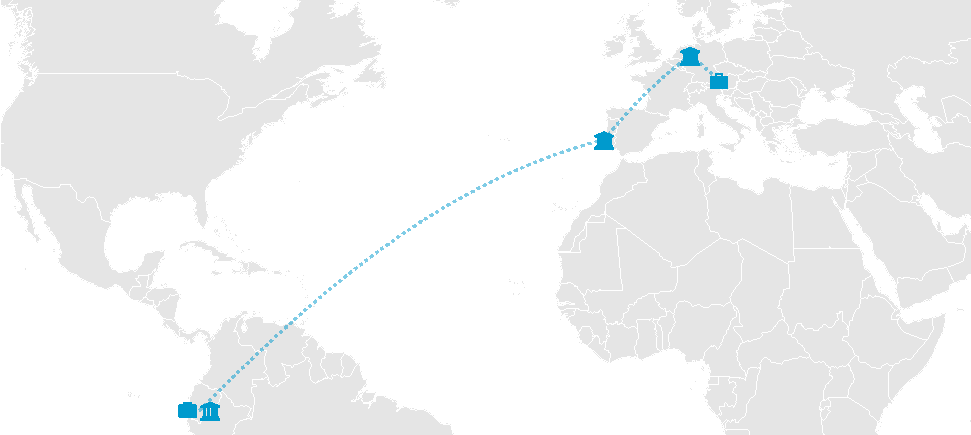
\includegraphics{CV_files/figure-latex/edu_plot-1} \end{center}

\hypertarget{professional-experience}{%
\section{\texorpdfstring{\faIcon{briefcase} Professional Experience}{ Professional Experience}}\label{professional-experience}}

\detailedsection{\detaileditem{University of Salzburg}{04, 2019 - Present}{Researcher - Department of Geoinformatics - Z\_GIS}{Salzburg, AT}{\item{Researcher for the MORPH, RiCoLa, STEC, citizenMORPH, MontEO projects in the Landslide division of the OBIA group.}}\detaileditem{Universidad de Cuenca}{05, 2017 - 08, 2017}{Research Assistant - Grupo de Investigación de Ciudades Sustentables Llactalab - Departamento Interdisciplinario de Espacio y Población}{Cuenca, EC}{\item{Spatio-temporal data analyst for the project: ``Study of Cyclists and Pedestrian Mobility Patterns in Cuenca for a Sustainable Mobility''.}}\detaileditem{Universidad de Cuenca}{09, 2016 - 08, 2017}{Technical Assistant - Carrera de Ingeniería Ambiental - Facultad de Ciencias Químicas}{Cuenca, EC}{\item{CEDIA project ``Geo-statistical Inference of Meteorological Data for Azuay and Chimborazo provinces''.}}\detaileditem{Universidad de Cuenca}{10, 2016 - 01, 2017}{Researcher - Carrera de Ingeniería Ambiental - Facultad de Ciencias Químicas}{Cuenca, EC}{\item{Project ``Water Quality and Environmental Variables Monitoring in Artificial Habitats for Endangered Species in Cuenca''.}}\detaileditem{Universidad de Cuenca}{03, 2016 - 07, 2016}{Research Assistant - Carrera de Ingeniería Ambiental - Facultad de ciencias Químicas}{Cuenca, EC}{\item{Project ``Determination of Particulate Matter PM10, PM2.5, and noise in Cuenca canton''.}}\detaileditem{Universidad de Cuenca}{05, 2015 - 06, 2015}{Intership - Grupo de Investigación de Ciudades Sustentables Llactalab - Departamento Interdisciplinario de Espacio y Población}{Cuenca, EC}{\item{Cartographic data gathering organization, topographic correction and categorization of urban land uses, scientific papers analysis for bibliographic review.}}\detaileditem{Universidad de Cuenca}{07, 2014 - 09, 2014}{Intership - Departamento de Recursos Hídricos y Ciencias Ambientales (iDRHICA)}{Cuenca, EC}{\item{Assess the functioning state of Davis Station sensors, identify similarities and differences of two river basins hydrograms, analyze the effects of temperature and relative humidity on reference evapotranspiration calculation.}}}

\pagebreak

\hypertarget{teaching-experience}{%
\section{\texorpdfstring{\faIcon{chalkboard} Teaching Experience}{ Teaching Experience}}\label{teaching-experience}}

\detailedsection{\detaileditem{Universidad de Cuenca}{03, 2015 - 07, 2015}{Teaching Assistant - Carrera de Ingeniería Ambiental - Facultad de Ciencias Químicas}{Cuenca, EC}{\item{Remote Sensing course for the Environmental Engineering Career from the University of Cuenca.}}\detaileditem{Universidad de Cuenca}{03, 2012 - 01, 2015}{Teaching Assistant - Carrera de Ingeniería Ambiental - Facultad de Ciencias Químicas}{Cuenca, EC}{\item{Introduction to Physics course for the Environmental Engineering Career from the University of Cuenca.}}}

\hypertarget{education}{%
\section{\texorpdfstring{\faIcon{university} Education}{ Education}}\label{education}}

\detailedsection{\detaileditem{Erasmus Mundus Msc. Geospatial Technologies}{2018 - 2019}{Westfälische Wilhelms-Universität Münster}{Münster, DE}{\item{S2 2018: covering Cartography, Reference Systems, Spatial Data Science with R, Unmanned Aerial Systems}\item{S3 2018: Masters Thesis: Validating a bike network analysis score based on open data as a connectivity measure of urban cycling infrastructure adapted for European cities. Supervised by Prof. Dr. Edzer Pebesma. URL: \textit{http://hdl.handle.net/10362/67511}}}\detaileditem{Erasmus Mundus Msc. Geospatial Technologies}{2017 - 2019}{Universidade Nova de Lisboa}{Lisbon, PT}{\item{S1, 2017: covering Geospatial Data Mining, Geostatistics, Remote Sensing, Geographic Information Science, Python programming.}\item{More info: \textit{https://mastergeotech.info/}}}\detaileditem{Environmental Engineer BSc.}{2011 - 2016}{Universidad de Cuenca}{Cuenca, EC}{\item{Covering Cartography, Remote Sensing, Ecology, Hydrology, Meteorology and Climatology, Environmental Studies, Natural Resources Management, among 66 subjects during 10 semesters.}\item{Bachelor Thesis (in spanish): Particulate Matter less than 10 microns concentration estimation through Remote Sensing in the Urban Area of Cuenca city. Supervised by Danilo Mejía Coronel. URL: \textit{http://dspace.ucuenca.edu.ec/handle/123456789/25484}}}}

\hypertarget{selected-publications}{%
\section{\texorpdfstring{\faIcon*{file} Selected Publications}{ Selected Publications}}\label{selected-publications}}

\detailedsection{\detaileditem{GSA 2020 Connects Online}{10, 2020}{Generation of Multi-Temporal Dems from Sentinel-1 for Assessing Geomorphological Changes in the Hítardalur Valley, Western Iceland}{Conference Proceedings}{\item{Dabiri, Z., Hölbling, D., \textbf{Abad, L.}, Helgason, J. K., Sæmundsson, Þ., Tiede, D. (2020). Generation of Multi-Temporal Dems from Sentinel-1 for Assessing Geomorphological Changes in the Hítardalur Valley, Western Iceland. Geological Society of America Abstracts with Programs, 52 (6). \textit{https://doi.org/10.1130/abs/2020AM-357105}}}\detaileditem{Applied Sciences}{08, 2020}{Assessment of Landslide-Induced Geomorphological Changes in Hítardalur Valley, Iceland, Using Sentinel-1 and Sentinel-2 Data}{Journal Article}{\item{Dabiri, Z., Hölbling, D., \textbf{Abad, L.}, Helgason, J. K., Sæmundsson, Þ., Tiede, D. (2020). Assessment of Landslide-Induced Geomorphological Changes in Hítardalur Valley, Iceland, Using Sentinel-1 and Sentinel-2 Data. Applied Sciences, 10(17), 5848. \textit{https://doi.org/10.3390/app10175848}}}\detaileditem{Journal for Geographic Information Science}{06, 2020}{Implementing Geo Citizen Science Solutions: Experiences from the citizenMorph Project}{Journal Article}{\item{Hennig, S., \textbf{Abad, L.}, Hölbling, D., Tiede, D. (2020). Implementing Geo Citizen Science Solutions : Experiences from the citizenMorph Project. Journal for Geographic Information Science, 7(2), 3–14. \textit{https://doi.org/10.1553/giscience2020}}}\detaileditem{Science of the Total Environment}{06, 2020}{Distinct types of landslides in moraines associated with the post-LIA glacier thinning: Observations from the Kinzl Glacier, Huascarán, Peru}{Journal Article}{\item{Emmer, A., Klimeš, J., Hölbling, D., \textbf{Abad, L.}, Draebing, D., Skalák, P., Štepánek, P., Zahradnícek, P. (2020). Distinct types of landslides in moraines associated with the post-LIA glacier thinning: Observations from the Kinzl Glacier, Huascarán, Peru. Science of The Total Environment, 739, 139997. \textit{https://doi.org/10.1016/j.scitotenv.2020.139997}}}\detaileditem{EGU General Assembly 2020}{03, 2020}{Mapping and monitoring of landslide-dammed lakes using Sentinel-2 time series -a case study after the 2016 Kaikoura Earthquake in New Zealand}{Conference Proceedings}{\item{\textbf{Abad, L.}, Hölbling, D., Spiekermann, R., Dabiri, Z., Prasicek, G., Argentin, A.-L. (2020). Mapping and monitoring of landslide-dammed lakes using Sentinel-2 time series -a case study after the 2016 Kaikoura Earthquake in New Zealand. EGU General Assembly 2020. \textit{https://doi.org/10.5194/egusphere-egu2020-572}}}\detaileditem{EGU General Assembly 2020}{03, 2020}{Assessing the impact of mass movements on alpine trails and huts using EO data.}{Conference Proceedings}{\item{Albrecht, F., Hölbling, D., \textbf{Abad, L.}, Dabiri, Z., Reischenböck, G., Hipp, T., Resch, H., Resch, G. (2020). Assessing the impact of mass movements on alpine trails and huts using EO data. EGU General Assembly 2020. \textit{https://doi.org/10.5194/egusphere-egu2020-21325}}}\detaileditem{Applied Sciences, MDPI}{01, 2020}{Mapping and Analyzing the Evolution of the Butangbunasi Landslide Using Landsat Time Series with Respect to Heavy Rainfall Events during Typhoons}{Journal Article}{\item{Hölbling, D., \textbf{Abad, L.}, Dabiri, Z., Prasicek, G., Tsai, T.-T., Argentin, A.-L. Mapping and Analyzing the Evolution of the Butangbunasi Landslide Using Landsat Time Series with Respect to Heavy Rainfall Events during Typhoons. Applied Sciences. 2020, 10, 630. \textit{https://doi.org/10.3390/app10020630}}}\detaileditem{Information, MDPI}{11, 2018}{Quantifying Bicycle Network Connectivity in Lisbon Using Open Data}{Journal Article}{\item{\textbf{Abad, L}., van der Meer, L. (2018). Quantifying Bicycle Network Connectivity in Lisbon Using Open Data. Information, 9(11), 14. \textit{https://doi.org/10.3390/info9110287}}}\detaileditem{Maskana}{06, 2018}{Exploratory analysis of volunteer cyclists behavior through spatio-temporal patterns mining in  Cuenca, Ecuador}{Journal Article}{\item{\textbf{Abad, L.}, Orellana, D. (2018). Análisis exploratorio de comportamientos de ciclistas voluntarios mediante minería de patrones espacio-temporales en Cuenca, Ecuador. Maskana, 9(1), 141-151.}}\detaileditem{XVI Conferencia de Sistemas de Información Geográfica}{09, 2017}{Particulate Matter less than 10 microns concentration estimation through Remote Sensing in the Urban Area of Cuenca city}{Conference Proceedings}{\item{\textbf{Abad, L.}, Mejía-Coronel, D. (2017). Estimación De La Concentración De Material Particulado Menor a 10 Micras a Través De Sensores Remotos En El Área Urbana De La Ciudad De Cuenca. In XVI Conferencia de Sistemas de Información Geográfica (pp. 381-390). Cuenca, Ecuador. Universidad del Azuay.}}}

\hypertarget{projects}{%
\section{\texorpdfstring{\faIcon{lightbulb} Projects}{ Projects}}\label{projects}}

\smallskip

\hypertarget{research-projects}{%
\subsection{\texorpdfstring{\faIcon{satellite} Research projects}{ Research projects}}\label{research-projects}}

\detailedsection{\detaileditem{Smarter Targeting of Erosion Control}{2018 - 2023}{STEC}{NZ}{\empty}\detaileditem{The impact of mass movements on alpine trails and huts assessed by EO data}{2020 - 2021}{MontEO \href{http://monteo.zgis.at/}{\tiny{\faIcon{link}}}}{AT}{\empty}\detaileditem{Detection and Analysis of Landslide-induced River Course Changes and Lake Formation}{2017 - 2020}{RiCoLa \href{http://landslides-and-rivers.sbg.ac.at/}{\tiny{\faIcon{link}}}}{AT, NZ, TW}{\empty}\detaileditem{Observation and Reporting of Landscape Dynamics by Citizens}{2018 - 2020}{citizenMorph \href{http://citizenmorph.sbg.ac.at/}{\tiny{\faIcon{link}}}}{AT, DE, IS}{\empty}\detaileditem{Mapping, Monitoring and Modelling the Spatio-Temporal Dynamics of Land Surface Morphology}{2016 - 2020}{MORPH \href{http://morph.sbg.ac.at/}{\tiny{\faIcon{link}}}}{IS}{\empty}}

\smallskip

\hypertarget{programming-projects}{%
\subsection{\texorpdfstring{\faIcon{laptop-code} Programming projects}{ Programming projects}}\label{programming-projects}}

\detailedsection{\detaileditem{Landslide dammed-lakes detection and monitoring after the Kaikoura earthquake in New Zealand}{}{Kaikoura landslide dammed-lakes \href{https://github.com/loreabad6/KaikouraDammedLakes_public}{\tiny{\faIcon{link}}}}{GEE project}{\empty}\detaileditem{Tidy Geospatial Networks in R}{}{sfnetworks \href{https://luukvdmeer.github.io/sfnetworks/}{\tiny{\faIcon{link}}}}{R Package}{\empty}\detaileditem{Bicycle Network Analysis Score for UK and NL}{}{BNA-EU \href{https://github.com/loreabad6/masters-thesis-geotech}{\tiny{\faIcon{link}}}}{RMarkdown Reporting}{\empty}}

\hypertarget{presentations-blogs-courses}{%
\section{\texorpdfstring{\faIcon{comments} Presentations, blogs, courses}{ Presentations, blogs, courses}}\label{presentations-blogs-courses}}

\detailedsection{\detaileditem{Lightning Talk at the Geo For Good 2020 Summit Public Sector Meetup \href{https://www.youtube.com/watch?v=CbHYkUpCwCI&ab_channel=GoogleEarth}{\tiny{\faIcon{link}}}}{10, 2020}{Mapping and monitoring landslide-dammed lakes in Kaikoura, New Zealand, using the Google Earth Engine}{Geo for Good 2020}{\empty}\detaileditem{Invited talk at the event 'Voces de la Ingeniería Ambiental' \href{https://loreabad6.github.io/VocesAmbiental/presentacion.html}{\tiny{\faIcon{link}}}}{09, 2020}{El rol de las tecnologías geoespaciales para el mapeo y monitoreo de peligros naturales}{Voces Ambiental 2020}{\empty}\detaileditem{Presentation during Cycling Potential Hackathon: Lisbon \href{https://github.com/U-Shift/cyclingpotential-hack}{\tiny{\faIcon{link}}}}{09, 2020}{Bicycle Network Analysis for assessing cyclability}{U-Shift event}{\empty}\detaileditem{Full paper presentation in session C43: Spatial Citizens Science \href{https://www.conftool.com/giweek2020/index.php?page=browseSessions&form_session=202}{\tiny{\faIcon{link}}}}{07, 2020}{Implementing geo citizen science solutions: experiences from the citizenMorph project}{Gi-Forum 2020}{\empty}\detaileditem{Webinar \& Hackathon \href{https://sfnetworks.github.io/sfnetworks-webinar/slides}{\tiny{\faIcon{link}}}}{06, 2020}{Tidy Geospatial Networks in R: Introducing the sfnetworks package}{e-Rum 2020 satellite event}{\empty}\detaileditem{Display in session Natural Hazards NH6.1 \href{https://presentations.copernicus.org/EGU2020/EGU2020-572_presentation.pdf}{\tiny{\faIcon{link}}}}{05, 2020}{Mapping and monitoring of landslide-dammed lakes using Sentinel-2 time series}{EGU 2020}{\empty}\detaileditem{R spatial crash course \href{https://luukvdmeer.github.io/maptimeR/exercises.html}{\tiny{\faIcon{link}}}}{02, 2020}{Intro to spatial vector data analysis with R}{Maptime Salzburg}{\empty}\detaileditem{Blogpost \href{https://www.r-spatial.org/r/2019/09/26/spatial-networks.html}{\tiny{\faIcon{link}}}}{09, 2019}{Spatial networks in R with sf and tidygraph}{r-spatial blog}{\empty}\detaileditem{Short Paper Presentation in the 2nd Open Data for Open Cities Workshop \href{https://github.com/GeoTecINIT/OpenData4OpenCities/blob/master/Presentations/AGILE_2018_Presentation_Abad-vdMeer.pdf}{\tiny{\faIcon{link}}}}{06, 2018}{Bicycle Network Analysis for Lisbon}{AGILE Workshop: OD4OC}{\empty}\detaileditem{Abstract Presentation}{11, 2017}{Exploring Space-Time Patterns Of Volunteered Cycling Data In An Intermediate City}{GeoMundus 2017}{\empty}}

\hypertarget{distinctions}{%
\section{\texorpdfstring{\faIcon{medal} Distinctions}{ Distinctions}}\label{distinctions}}

\briefsection{\briefitem{Benigno Malo Prize - University Honors Award}{2018}{Universidad de Cuenca}\briefitem{AGILE 2018 conference - travel grant}{2018}{AGILE \& ESRI}\briefitem{Erasmus Mundus Scholarship}{2017}{European Commission}\briefitem{Best Scientific Poster - 2nd International Summer School \newline 
``The Biodiversity of Genes, Species and Ecosystems''}{2015}{Universität Osnabrück}\briefitem{Vanguardia Honors Program}{2014 - 2016}{Universidad de Cuenca}}

\hypertarget{memberships}{%
\section{\texorpdfstring{\faIcon{users} Memberships}{ Memberships}}\label{memberships}}

\briefsection{\briefitem{R-Ladies Global \href{https://rladies.org/austria-rladies/name/lorena-abad/}{\tiny{\faIcon{link}}}}{since 2020}{}\briefitem{Women in Geospatial \href{https://speakers.womeningeospatial.org/speakers}{\tiny{\faIcon{link}}}}{since 2020}{}\briefitem{European Geosciences Union}{2020}{}\briefitem{Erasmus Mundus Association}{since 2020}{}}

\hypertarget{skills}{%
\section{\texorpdfstring{\faIcon{brain} Skills}{ Skills}}\label{skills}}

\smallskip

\hypertarget{technical-skills}{%
\subsection{\texorpdfstring{\faIcon{cogs} Technical skills}{ Technical skills}}\label{technical-skills}}

\detailedsection{\detaileditem{R -- SQL -- Python -- JavaScript}{}{Coding Languages}{}{\empty}\detaileditem{QGIS -- ArcGIS -- SAGA -- eCognition -- PostgreSQL -- PostGIS -- RStudio --  Earth Engine -- GIMP -- Mendeley}{}{Software}{}{\empty}\detaileditem{Git -- Markdown -- LaTex -- OpenStreetMap}{}{Other}{}{\empty}}

\smallskip

\hypertarget{organizational-skills}{%
\subsection{\texorpdfstring{\faIcon{calendar} Organizational skills}{ Organizational skills}}\label{organizational-skills}}

\briefsection{\briefitem{e-Rum 2020 satellite event: \textit{sfnetworks} Webinar and Hackathon \href{https://2020.erum.io/program/hackathon/}{\tiny{\faIcon{link}}}}{06, 2020}{Online Event}\briefitem{citizenMorph App Testing Workshop}{09, 2019}{Höfn, IS}\briefitem{GeoMundus 2018 \href{http://www.geomundus.org/2018/}{\tiny{\faIcon{link}}}}{12, 2018}{Lisbon, PT}\briefitem{I University Simposium of Environmental Science Research}{06, 2016}{Cuenca, EC}\briefitem{Vicepresident of the Student Association of Environmental Engineers}{2013 - 2014}{Cuenca, EC}}

\smallskip

\hypertarget{languages}{%
\subsection{\texorpdfstring{\faIcon{language} Languages}{ Languages}}\label{languages}}

\begin{table}[H]
\centering\begingroup\fontsize{9}{11}\selectfont

\begin{tabular}{>{\centering\arraybackslash}p{2.4cm}>{\centering\arraybackslash}p{2.4cm}>{\centering\arraybackslash}p{2.4cm}>{\centering\arraybackslash}p{2.4cm}>{\centering\arraybackslash}p{2.4cm}>{\centering\arraybackslash}p{2.4cm}c}
\toprule
Skill & Spanish & English & French & Portuguese & German & Dutch\\
\midrule
Reading & \textcolor[HTML]{005c7b}{Native} & \textcolor[HTML]{009acd}{C2} & \textcolor[HTML]{4cb8dc}{B2} & \textcolor[HTML]{4cb8dc}{B1} & \textcolor[HTML]{7fcce6}{A2} & \textcolor[HTML]{7fcce6}{A2}\\
Writing & \textcolor[HTML]{005c7b}{Native} & \textcolor[HTML]{009acd}{C1} & \textcolor[HTML]{4cb8dc}{B2} & \textcolor[HTML]{4cb8dc}{B1} & \textcolor[HTML]{7fcce6}{A1} & \textcolor[HTML]{7fcce6}{A1}\\
Listening & \textcolor[HTML]{005c7b}{Native} & \textcolor[HTML]{009acd}{C2} & \textcolor[HTML]{4cb8dc}{B2} & \textcolor[HTML]{4cb8dc}{B1} & \textcolor[HTML]{7fcce6}{B1} & \textcolor[HTML]{7fcce6}{A2}\\
Speaking & \textcolor[HTML]{005c7b}{Native} & \textcolor[HTML]{009acd}{C2} & \textcolor[HTML]{4cb8dc}{B2} & \textcolor[HTML]{4cb8dc}{B1} & \textcolor[HTML]{7fcce6}{B1} & \textcolor[HTML]{7fcce6}{A2}\\
\bottomrule
\multicolumn{7}{l}{\textit{ } \tiny Common European Framework of Reference for Languages: A1/A2: Basic User. B1/B2: Independent User. C1/C2: Proficient User}\\
\end{tabular}
\endgroup{}
\end{table}

\end{document}
